\section{Einleitung}
\subsection{Ziel der Praxisarbeit}
Gegenstand dieser Praxisarbeit ist die technische Analyse moderner Command-and-Control-Frameworks (C2) im Kontext von Red-Team-Operationen. Im Fokus stehen dabei Architekturkonzepte, Kommunikationsmechanismen sowie operative Eigenschaften aktueller C2-Lösungen. Exemplarisch wird das Framework Sliver detailliert untersucht und mit weiteren etablierten Frameworks wie Metasploit und Cobalt Strike vergleichend eingeordnet.\newline\newline
Auf Basis dieser Analyse werden die Einsatzmöglichkeiten moderner C2-Frameworks im Rahmen realitätsnaher Angriffssimulationen bewertet. Dabei werden sowohl technische Kriterien als auch operationelle Gesichtspunkte wie Skalierbarkeit, Flexibilität und Stealth betrachtet. Die gewonnenen Erkenntnisse dienen als Grundlage für die Einordnung des praktischen Nutzens von C2-Infrastrukturen in professionellen Sicherheitsprüfungen und im Kontext angebotener Penetrationstests.
\subsection{Einordnung von Command-and-Control (C2) im Red Teaming}
Im Red Teaming stellt Command-and-Control eine zentrale Phase innerhalb der Cyber Kill Chain\cite{microsoft2026cyberkillchain} dar. Nach erfolgreicher Kompromittierung eines Zielsystems ermöglicht eine C2-Infrastruktur die fortlaufende Steuerung kompromittierter Systeme, die Durchführung weiterer Aktionen sowie die Koordination komplexer Angriffsszenarien. Ohne eine funktionierende C2-Kommunikation ist eine nachhaltige und realitätsnahe Simulation moderner Angreifer nicht möglich.\newline
\begin{figure}[H]
\centering
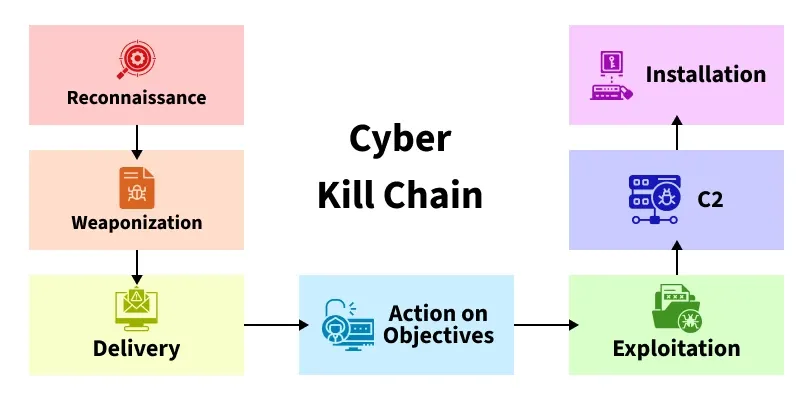
\includegraphics[width=\textwidth]{IMG/cyber_kill_chain.png}
\caption{Cyber Kill Chain}
\label{Cyber Kill chain}
\end{figure}
Im Gegensatz zu klassischen Penetrationstests, die häufig auf die Identifikation einzelner Schwachstellen fokussiert sind, zielt Red Teaming auf die Nachbildung vollständiger Angriffsabläufe ab. C2-Frameworks übernehmen hierbei die Rolle der zentralen Steuerungsinstanz und bilden die technische Grundlage für Post-Exploitation-Aktivitäten, laterale Bewegungen und persistente Zugriffsmechanismen. Ihre Ausgestaltung beeinflusst maßgeblich die Realitätsnähe und Aussagekraft einer Red-Team-Operation.
\subsection{Relevanz moderner C2-Frameworks für realistische Angreifersimulationen}
Moderne IT-Infrastrukturen sind zunehmend durch fortschrittliche Sicherheitsmechanismen wie Endpoint Detection and Response (EDR), Netzwerküberwachung und verhaltensbasierte Erkennungsverfahren geschützt. Vor diesem Hintergrund gewinnen leistungsfähige und flexibel einsetzbare C2-Frameworks eine besondere Bedeutung, da sie es ermöglichen, das Verhalten realer Angreifer realitätsnah abzubilden und bestehende Sicherheitsmaßnahmen gezielt zu evaluieren.
\newline\newline
Für die Abteilung Service Zentralbereich Cyber-Security (SZC) der ABB ergibt sich daraus ein direkter Mehrwert, da im Rahmen der angebotenen Sicherheitsdienstleistungen, insbesondere bei Penetrationstests, eine realistische Angreifersimulation zunehmend an Bedeutung gewinnt. Der Einsatz moderner C2-Frameworks erlaubt es, über rein punktuelle Schwachstellenanalysen hinauszugehen und die Widerstandsfähigkeit von Systemen und Prozessen gegenüber fortgeschrittenen Angriffsszenarien zu bewerten.
\newline\newline
Die in dieser Praxisarbeit untersuchten C2-Frameworks tragen somit dazu bei, die Qualität und Aussagekraft von Penetrationstests als Serviceleistung zu erhöhen und bilden zugleich eine technische Grundlage für weiterführende Fragestellungen, beispielsweise im Bereich der Tarnung von Payloads und Kommunikationsmustern. Diese Aspekte stellen eine sinnvolle Überleitung zu vertiefenden Untersuchungen in nachfolgenden Praxisphasen dar.